\documentclass[../piano_di_progetto.tex]{subfiles}

\begin{document}

In questa sezione verrà descritto come \emph{SpaghettiCode} intende usare le risorse a disposizione. \\
Per aiutare nella comprensione della tabella qui di seguito sono spiegate le sigle che verranno usate:
\begin{itemize}
\item \textbf{Re}: Responsabile;
\item \textbf{Am}: Amministratore;
\item \textbf{An}: Analista;
\item \textbf{Pg}: Progettista;
\item \textbf{Pr}: Programmatore;
\item \textbf{Ve}: Verificatore;
\end{itemize}


\subsection{ Fase di analisi}%
\label{sub:fase_analisi}
\subsubsection{Prospetto Orario}


\begin{table}[!ht]
	\centering
	\begin{tabular}{|l|c|c|c|c|c|c|c|}
	\hline
	\rowcolor{lightgray}
	\textbf{Nome} & \textbf{Re} & \textbf{Am} & \textbf{An} & \textbf{Pg}  & \textbf{Pr}   & \textbf{Ve} & \textbf{Totale}\\
	\hline
		Contro Daniel Eduardo & 0 & 0 & 13 & 0 & 0 & 14 & 27 \\
	\hline
		Fichera Jacopo & 0 & 0 & 13 & 0 & 0 & 14 & 27 \\
	\hline
		Kostadinov Samuel & 0 & 10 & 5 & 0 & 0 & 12 & 27 \\			
	\hline
		Masevski Martin & 4 & 10 & 5 & 0 & 0 & 8 & 27 \\
	\hline
		Pagotto Manuel & 0 & 0 & 13 & 0 & 0 & 14 & 27 \\			
	\hline
		Paparazzo Giorgia & 13 & 0 & 4 & 0 & 0 & 10 & 27 \\
	\hline
		Rizzo Stefano & 0 & 0 & 12 & 0 & 0 & 15 & 27 \\
	\hline	
	\end{tabular}
	\caption{Tabella contenente la suddivisione delle ore nella fase di Analisi}
\end{table}

\begin{figure}[H]
\centering
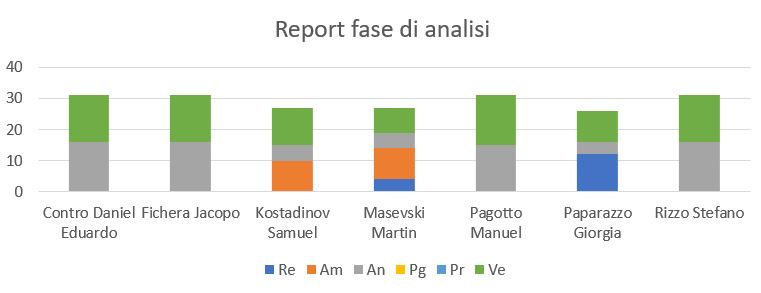
\includegraphics[width=12cm]{componenti/img/report_analisi}
\caption{Report della suddivisione dei ruoli nella fase di analisi}
\end{figure}

\newpage

\subsubsection{Prospetto Economico}


\begin{longtable}{|l|c|c|c|c|c|c|c|}
	\hline
	\rowcolor{lightgray}
	\textbf{Ruolo} & \textbf{Ore} & \textbf{Costo in €}\\
	\endhead
	\hline
	Responsabile & 17 & 510,00 \\
	\hline
	Amministratore & 20 & 400,00 \\
	\hline
	Analista & 65 & 1.625,00 \\
	\hline
	Progettista & 0 & 0 \\
	\hline
	Programmatore & 0 & 0 \\
	\hline
	Verificatore & 87 & 1.305,00 \\
	\hline
	\textbf{Totale} & 189 & 3.840,00 \\
	\hline
	\rowcolor{white}
	\caption{Tabella contenente il prospetto economico in riferimento al prospetto orario nella fase di Analisi} 
\end{longtable}


\subsection{ Fase di consolidamento requisiti}%
\label{sub:fase_cons}
\subsubsection{Prospetto Orario}

\begin{table}[!ht]

	\centering
	\begin{tabular}{|l|c|c|c|c|c|c|c|}
	\hline
	\rowcolor{lightgray}
	\textbf{Nome} & \textbf{Re} & \textbf{Am} & \textbf{An} & \textbf{Pg}  & \textbf{Pr}   & \textbf{Ve} & \textbf{Totale} \\
	\hline
		Contro Daniel Eduardo & 0 & 0 & 5 & 0 & 0 & 0  & 5 \\
	\hline
		Fichera Jacopo & 0 & 0 & 5 & 0 & 0 & 0 & 5 \\
	\hline
		Kostadinov Samuel & 0 & 1 & 4 & 0 & 0 & 0 & 5 \\			
	\hline
		Masevski Martin & 1 & 1 & 0 & 0 & 0 & 0 & 5 \\
	\hline
		Pagotto Manuel & 0 & 0 & 13 & 0 & 0 & 13 & 5 \\			
	\hline
		Paparazzo Giorgia & 1 & 0 & 0 & 0 & 0 & 0 & 5 \\
	\hline
		Rizzo Stefano & 0 & 0 & 5 & 0 & 0 & 0 & 5 \\
	\hline	
	\end{tabular}
	\caption{Tabella contenente la suddivisione delle ore nella fase di consolidamento}
\end{table}

\begin{figure}[H]
\centering
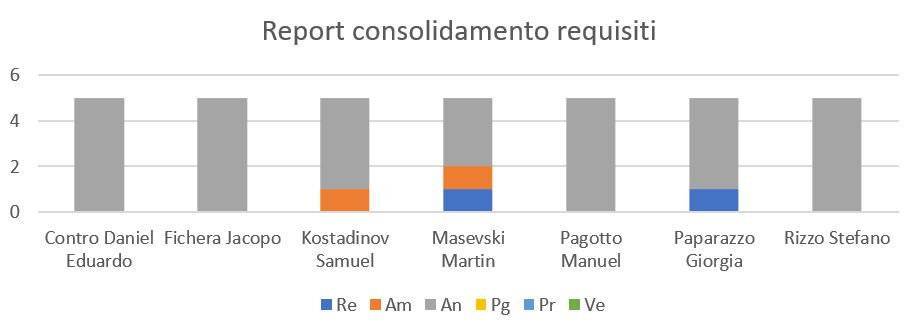
\includegraphics[width=12cm]{componenti/img/report_consolidamento}
\caption{Report della suddivisione dei ruoli nella fase di consolidamento}
\end{figure}

\subsubsection{Prospetto Economico}

\begin{longtable}{|l|c|c|c|c|c|c|c|}
	\hline
	\rowcolor{lightgray}
	\textbf{Ruolo} & \textbf{Ore} & \textbf{Costo in €}\\
	\endhead
	\hline
	Responsabile & 2 & 60,00 \\
	\hline
	Amministratore & 19 & 40,00 \\
	\hline
	Analista & 31 & 775,00 \\
	\hline
	Progettista & 0 & 0 \\
	\hline
	Programmatore & 0 & 0 \\
	\hline
	Verificatore & 0 & 0 \\
	\hline
	\textbf{Totale} & 35 & 875,00 \\
	\hline
	\rowcolor{white}
	\caption{Tabella contenente il prospetto economico in riferimento al prospetto orario nella fase di consolidamento} 
\end{longtable}


\subsection{ Fase di progettazione architetturale}%
\label{sub:fase_prog_arc}
\subsubsection{Prospetto Orario}

\begin{center}
	\begin{longtable}{|l|c|c|c|c|c|c|c|}
		\hline
		\rowcolor{lightgray}
		\textbf{Nome} & \textbf{Re} & \textbf{Am} & \textbf{An} & \textbf{Pg}  & \textbf{Pr}   & \textbf{Ve} & \textbf{Totale} \\

		\hline
			Contro Daniel Eduardo & 0 & 7 & 0 & 8 & 6 & 9 & 30\\
		\hline
			Fichera Jacopo & 0 & 0 & 0 & 10 & 7 & 13 & 30 \\
		\hline
			Kostadinov Samuel & 0 & 0 & 8 & 8 & 0 & 14 & 30 \\			
		\hline
			Masevski Martin 	& 11 & 0 & 0 & 0 & 5 & 14 & 30\\
		\hline
			Pagotto Manuel & 10 & 0 & 9 & 0 & 0 & 11 & 30 \\			
		\hline
			Paparazzo Giorgia & 0 & 0 & 10 & 4 & 6 & 10 & 30 \\
		\hline
			Rizzo Stefano & 0 & 9 & 0 & 4 & 4 & 13 & 30\\
		\hline	
		\rowcolor{white}
		\caption{Tabella contenente la suddivisione delle ore nella fase di Progettazione Architetturale}
	\end{longtable}
\end{center}

\begin{figure}[H]
\centering
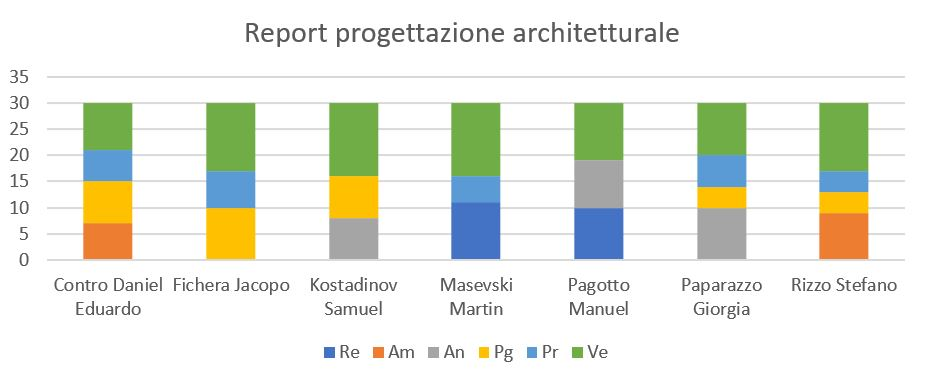
\includegraphics[width=12cm]{componenti/img/report_prog_arc}
\caption{Report della suddivisione dei ruoli nella fase di progettazione architetturale}
\end{figure}

\subsubsection{Prospetto Economico}

\begin{center}
	\begin{longtable}{|l|c|c|c|c|c|c|c|}
		\hline
		\rowcolor{lightgray}
		\textbf{Ruolo} & \textbf{Ore} & \textbf{Costo in €}\\

		\hline
		Responsabile & 21 & 630,00\\
		\hline
		Amministratore & 16 & 320,00\\
		\hline
		Analista & 27 & 675,00\\
		\hline
		Progettista & 34 & 748,00\\
		\hline
		Programmatore & 28 & 420,00\\
		\hline
		Verificatore & 84 & 1.260,00\\
		\hline
		\textbf{Totale} & 210 & 4.053,00\\
		\hline
		\rowcolor{white}
		\caption{Tabella contenente il prospetto economico in riferimento al prospetto orario nella fase di Progettazione architetturale}
	\end{longtable}
\end{center}

\subsection{ Fase di progettazione di dettaglio}%
\label{sub:fase_prog_dett}
\subsubsection{Prospetto Orario}

\begin{center}
	\begin{longtable}{|l|c|c|c|c|c|c|c|}
		\hline
		\rowcolor{lightgray}
		\textbf{Nome} & \textbf{Re} & \textbf{Am} & \textbf{An} & \textbf{Pg}  & \textbf{Pr}   & \textbf{Ve} & \textbf{Totale} \\

		\hline
			Contro Daniel Eduardo & 9 & 0 & 0 & 10 & 18 & 13 & 50 \\
		\hline
			Fichera Jacopo & 0 & 0 & 0 & 17 & 17 & 16 & 50 \\
		\hline
			Kostadinov Samuel & 10 & 0 & 0 & 8 & 15 & 17 & 50 \\			
		\hline
			Masevski Martin & 0 & 0 & 5 & 13 & 13 & 19 & 50 \\
		\hline
			Pagotto Manuel & 8 & 0 & 0 & 9 & 16 & 17 & 50 \\		
		\hline
			Paparazzo Giorgia & 0 & 6 & 2 & 17 & 10 & 15 & 50 \\
		\hline
			Rizzo Stefano & 0 & 8 & 0 & 12 & 14 & 16 & 50 \\
		\hline	
		\rowcolor{white}
		\caption{Tabella contenente la suddivisione delle ore nella fase di Progettazione di dettaglio}
	\end{longtable}
\end{center}

\begin{figure}[H]
\centering
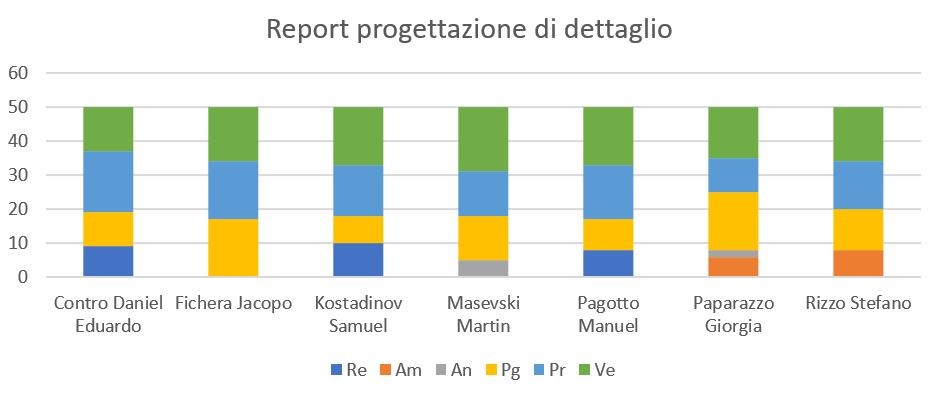
\includegraphics[width=12cm]{componenti/img/report_prog_dett}
\caption{Report della suddivisione dei ruoli nella fase di progettazione di dettaglio}
\end{figure}

\newpage

\subsubsection{Prospetto Economico}

\begin{center}
	\begin{longtable}{|l|c|c|c|c|c|c|c|}
		\hline
		\rowcolor{lightgray}
		\textbf{Ruolo} & \textbf{Ore} & \textbf{Costo in €}\\
		\hline
		Responsabile & 27 & 810,00\\
		\hline
		Amministratore & 14 & 280,00\\
		\hline
		Analista & 7 & 175,00\\
		\hline
		Progettista & 86 & 1.892,00\\
		\hline
		Programmatore & 103 & 1.545,00\\
		\hline
		Verificatore & 113 & 1.695,00\\
		\hline
		\textbf{Totale} & 350 & 6.397,00\\
		\hline
		\rowcolor{white}
		\caption{Tabella contenente il prospetto economico in riferimento al prospetto orario nella fase di Progettazione di dettaglio}
	\end{longtable}
\end{center}

\subsection{ Fase di validazione e collaudo}%
\label{sub:fase_valid_collaudo}
\subsubsection{Prospetto Orario}

\begin{center}
	\begin{longtable}{|l|c|c|c|c|c|c|c|}
		\hline
		\rowcolor{lightgray}
		\textbf{Nome} & \textbf{Re} & \textbf{Am} & \textbf{An} & \textbf{Pg}  & \textbf{Pr}   & \textbf{Ve} & \textbf{Totale} \\

		\hline
			Contro Daniel Eduardo & 0 & 0 & 0 & 0 & 0 & 13 & 20\\
		\hline
			Fichera Jacopo & 9 & 4 & 0 & 0 & 0 & 7 & 20 \\ 
		\hline
			Kostadinov Samuel & 0 & 0 & 0 & 10 & 2 & 8 & 20 \\ 		
		\hline
			Masevski Martin & 0 & 0 & 0 & 5 & 0 & 15 & 20 \\
		\hline
			Pagotto Manuel & 0 & 4 & 0 & 6 & 0 & 10 & 20 \\			
		\hline
			Paparazzo Giorgia & 0 & 0 & 0 & 4 & 0 & 12 & 20 \\
		\hline
			Rizzo Stefano & 8 & 0 & 2 & 0 & 0 & 10 & 20 \\
		\hline	
		\rowcolor{white}
		\caption{Tabella contenente la suddivisione delle ore nella fase di Validazione e collaudo}
	\end{longtable}
\end{center}

\begin{figure}[H]
\centering
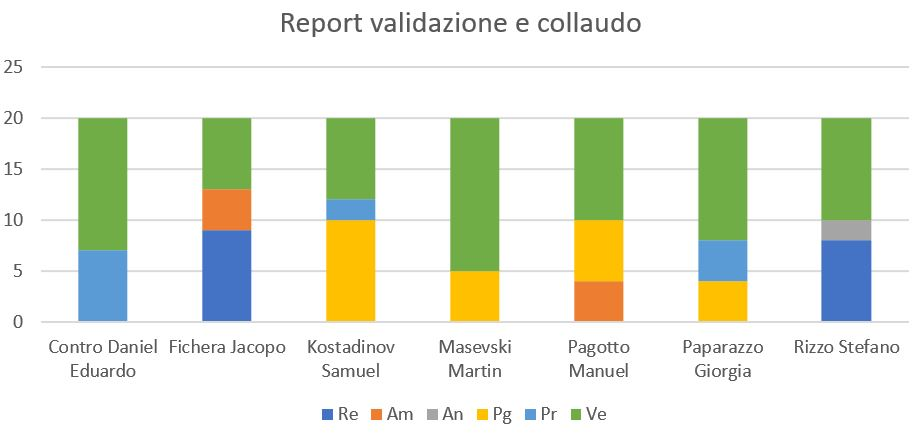
\includegraphics[width=12cm]{componenti/img/report_valid_collaudo}
\caption{Report della suddivisione dei ruoli nella fase di validazione e collaudo}
\end{figure}

\subsubsection{Prospetto Economico}

\begin{center}
	\begin{longtable}{|l|c|c|c|c|c|c|c|}
		\hline
		\rowcolor{lightgray}
		\textbf{Ruolo} & \textbf{Ore} & \textbf{Costo in €}\\

		\hline
		Responsabile & 17 & 510,00\\
		\hline
		Amministratore & 8 & 160,00\\
		\hline
		Analista & 2 & 50,00\\
		\hline
		Progettista & 25 & 550,00\\
		\hline
		Programmatore & 13 & 195,00\\
		\hline
		Verificatore & 75 & 1.125,00\\
		\hline
		\textbf{Totale} & 140 & 2.590,00\\
		\hline
		\caption{Tabella contenente il prospetto economico in riferimento al prospetto orario nella fase di Validazione e collaudo}
	\end{longtable}
\end{center}

\newpage

\subsection{Riepilogo}%
\label{sub:riepilog}
Nella seguente tabella viene riportato il riepilogo delle ore impiegate, incluse le ore svolte in fase di analisi e di studio personale: \\

\textbf{Prospetto Orario}

\begin{center}
	\begin{longtable}{|l|c|c|c|c|c|c|c|}
		\hline
		\rowcolor{lightgray}
		\textbf{Nome} & \textbf{Re} & \textbf{Am} & \textbf{An} & \textbf{Pg}  & \textbf{Pr}   & \textbf{Ve} & \textbf{Totale} \\

		\hline
			Contro Daniel Eduardo & 9 & 7 & 18 & 18 & 31 & 49 & 132 \\
		\hline
			Fichera Jacopo & 9 & 4 & 18 & 27 & 24 & 50 & 132 \\
		\hline
			Kostadinov Samuel & 10 & 11 & 17 & 26 & 17 & 51 & 132 \\
		\hline
			Masevski Martin & 16 & 11 & 13 & 18 & 18 & 56 & 132 \\
		\hline
			Pagotto Manuel & 18 & 4 & 27 & 15 & 16 & 52 & 132 \\			
		\hline
			Paparazzo Giorgia & 14 & 6 & 20 & 25 & 20 & 47 & 132 \\
		\hline
			Rizzo Stefano & 8 & 17 & 19 & 16 & 18 & 54 & 132 \\
		\hline	
		\rowcolor{white}
		\caption{Tabella contenente il totale delle ore impiegate, non rendicontate}
	\end{longtable}
\end{center}

\begin{figure}[H]
\centering
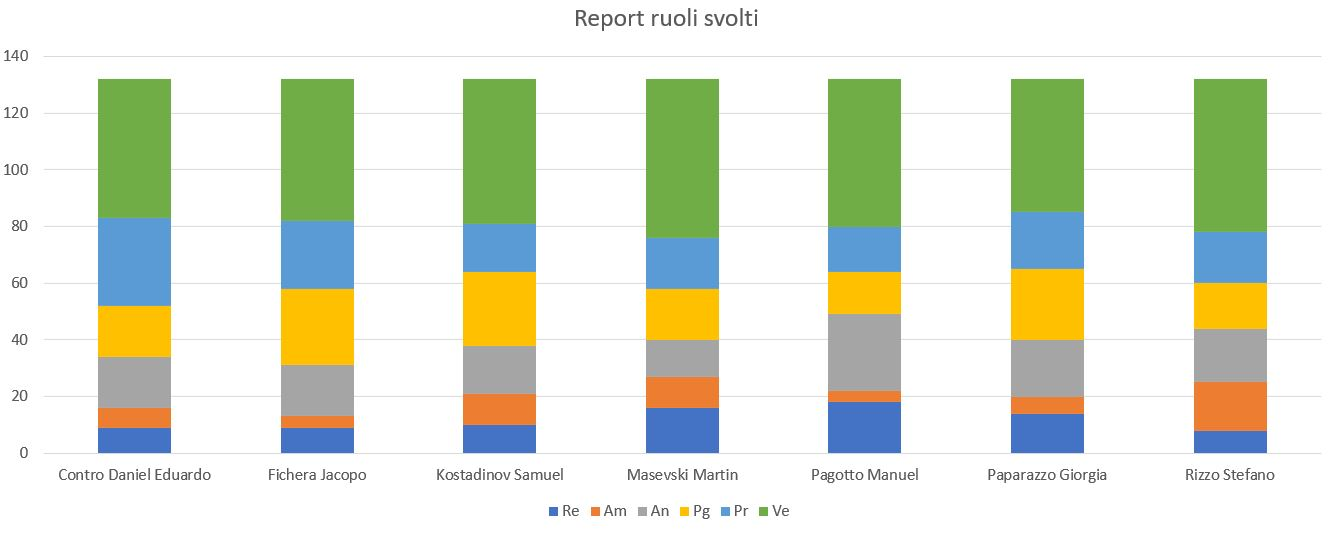
\includegraphics[width=12cm]{componenti/img/report_ruoli_tot}
\caption{Report della suddivisione dei ruoli nel totale del progetto, incluso le ore non rendicontate}
\end{figure}

\textbf{Prospetto Economico}

\begin{center}
	\begin{longtable}{|l|c|c|c|c|c|c|c|}
		\hline
		\rowcolor{lightgray}
		\textbf{Ruolo} & \textbf{Ore} & \textbf{Costo in €}\\

		\hline
		Responsabile & 2.460,00 & 82 \\
		\hline
		Amministratore & 1.160,00 & 58 \\
		\hline
		Analista & 2.525,00 & 101 \\
		\hline
		Progettista & 3.190,00 & 145 \\
		\hline
		Programmatore & 2.160,00 & 144 \\
		\hline
		Verificatore & 5.385,00 & 359 \\
		\hline
		\textbf{Totale} & \textbf{889} & \textbf{17.755,00}\\
		\hline

		\caption{Tabella contenente il prospetto economico in riferimento al totale delle ore impiegate, non rendicontate}
	\end{longtable}
\end{center}


Di seguito invece viene riportato il prospetto rendicontato:\\

\textbf{Prospetto Orario}

\begin{center}
	\begin{longtable}{|l|c|c|c|c|c|c|c|}
		\hline
		\rowcolor{lightgray}
		\textbf{Nome} & \textbf{Re} & \textbf{Am} & \textbf{An} & \textbf{Pg}  & \textbf{Pr}   & \textbf{Ve} & \textbf{Totale} \\

		\hline
			Contro Daniel Eduardo & 9 & 7 & 0 & 18 & 31 & 35 & 100 \\
		\hline
			Fichera Jacopo & 9 & 4 & 0 & 27 & 24 & 36 & 100 \\
		\hline
			Kostadinov Samuel & 10 & 0 & 8 & 26 & 17 & 39 & 100 \\		
		\hline
			Masevski Martin & 11 & 0 & 5 & 18 & 18 & 48 & 100 \\
		\hline
			Pagotto Manuel & 18 & 4 & 9 & 15 & 16 & 38 & 100 \\			
		\hline
			Paparazzo Giorgia & 0 & 6 & 12 & 25 & 20 & 37 & 100 \\
		\hline
			Rizzo Stefano & 8 & 17 & 2 & 16 & 18 & 39 & 100 \\
		\hline	
		\rowcolor{white}
		\caption{Tabella contenente il totale delle ore impiegate rendicontate}
	\end{longtable}
\end{center}

\textbf{Prospetto Economico}

\begin{center}
	\begin{longtable}{|l|c|c|c|c|c|c|c|}
		\hline
		\rowcolor{lightgray}
		\textbf{Ruolo} & \textbf{Ore} & \textbf{Costo in €}\\

		\hline
		Responsabile & 65 & 1.950,00 \\
		\hline
		Amministratore & 38 & 760,00 \\
		\hline
		Analista & 36 & 900,00 \\
		\hline
		Progettista & 145 & 3.190,00 \\
		\hline
		Programmatore & 144 & 2.160,00 \\
		\hline
		Verificatore & 272 & 4.080,00 \\
		\hline
		\textbf{Totale} & \textbf{700} & \textbf{13.040,00}\\
		\hline
		\caption{Tabella contenente il prospetto economico in riferimento al totale delle ore impiegate rendicontate}
	\end{longtable}
\end{center}

\end{document}